\documentclass{ctexart}
\usepackage{amsmath}
\usepackage{float}
\usepackage{amssymb}
\usepackage{graphicx}
\usepackage{gbt7714}
\usepackage{pifont}
\usepackage{wrapfig}
\usepackage{multirow}
\usepackage{array}

\ctexset{
    % 修改 section。
    section={   
        name={,、},
        number={\chinese{section}}
    }
}

\title{液体比热容的测量}
\author{陆知辰-10225301478}
\date{\today}
\graphicspath{{figure/}}

\begin{document}

\begin{titlepage}
  \centering
  % 插入图片
  
\includegraphics[width=0.5\textwidth]{ecnu.png}
  
  % 空行用于调整标题位置
  \vspace*{\baselineskip}
  
  % 标题
  \Huge\textbf{物\quad 理\quad 实\quad 验 \quad (二)}
  % 空行用于调整标题和其他信息之间的间距
  \vspace*{0.3\baselineskip}
  
  % 具体实验名称
  \huge 液体比热容的测量
  
  % 空行用于调整时间和其他信息之间的间距
  \vspace*{2\baselineskip}
  
  % 时间
  \large 时间:\today
  
  % 空行用于调整时间和其他信息之间的间距
  \vspace*{\baselineskip}
  
  % 创作人
  \large 创作人:陆知辰
  
  % 空行用于调整创作人和学号之间的间距
  \vspace*{\baselineskip}
  
  % 学号
  \large 学号:10225301478
  
\end{titlepage}
\newpage
\tableofcontents
\newpage
\section{实验摘要}
  \subsection{实验概要}
  比热容是热学中一个重要的物理量,物质比热容的测量是物理学的基本测量之一,
  对于了解物质的结构、确定物质的相变以及新能源的开发和新材料的研制等方面,都起着重要作用。
  测量液体比热容的方法有电加热法、冷却法、辐射法、混合法、比较法等。本实验采用比较法测量饱和食盐水的比热容。

  \subsection{实验目的}
  1.\quad 了解学会用冷却法和比较法测量液体的比热容,并了解比较法的使用条件。

  2.\quad 学会用实验的方法考察热学系统的冷却速率同系统与环境间温度差之间的关系。
  
  3.\quad 了解冷却法所用仪器设计的依据,能够从降低误差的角度规划液体体积、拟定操作步骤。

\section{实验原理}
  由牛顿冷却定律可知,一个表面温度为$\theta$的物体,在温度为$\theta_{0}$的环境中
  自然冷却$(\theta > \theta_{0})$,
  在单位时间里物体散失的热量$\delta Q / \delta t$与温度差$\theta - \theta_{0}$有下列关系:

  \begin{equation}
    \frac{\delta Q}{\delta t} = k (\theta - \theta_{0})
  \end{equation}

  设物质的热容为$C_{s}$,在散失热量$\delta Q$后,温度改变量为$\delta \theta$,
  则$\delta Q = C_{s} \delta \theta$.
  当物体温度的变化是准静态过程时,上式可改写为
  
  \begin{equation}
    \frac{\delta \theta}{\delta t} = \frac{k}{C_{s}} (\theta-\theta_{0})
  \end{equation}

  其中$\delta \theta / \delta t$为物体的冷却速率,$C_{s}$为物质的热容,$k$为物体的散热常数,
  与物体的表面性质、表面积、物体周围介质的性质和状态以及物体表面温度等许多因素有关,
  $\theta$和$\theta_{0}$分别为物体的温度和环境的温度。
  k为负数,$\theta 0-\theta_{0}$的数值应该很小,在10~15$^{\circ} C$之间。

  如果在实验中使环境温度$\theta$保持恒定,则可以认为$\theta$是常量,对上式进行积分,可以得到

  \begin{equation}
    ln(\theta - \theta_{0}) = \frac{k}{C_{s}} t + b
  \end{equation}
  式子中的b为常数

  可以将上式看成为两个变量的线性方程:自变量为t
  因变量为$ln(\theta - \theta_{0})$直线斜率为$k/C_{s}$.对于待测液体,
  它的散热系数k和热容$C_{s}$是未知的,因而只是依靠待测液体的温度曲线难以获得待测液体的比热容,
  为此,需要采用比较法开展实验.对两个实验系统在相同的实验条件下进行对比,
  从而确定未知物理量的方法,叫作比较法。
  
  比较法作为一种实验方法,有广泛的应用。在本实验中,将纯净水作为标准液体,
  饱和食盐水作为待测液体,在实验中用同一个容器分别盛水和盐水,
  在这两种情况下保持系统的初始温度、表面积和环境温度等基本相同,
  则系统盛水和盐水时的系数$k^{'}$与$k^{''}$相等,即

  $$k^{'} = k^{''} = k$$

  分别写出对已知标准液体(即纯净水)和待测液体(即饱和食盐水)进行冷却的公式,如下:

  \begin{equation}
  \left\{  
  \begin{aligned}
      & ln(\theta - \theta_{0}) _{w} = \frac{k^{'}}{C^{'}_{s}} t + b^{'} \\
      & ln(\theta - \theta_{0}) _{s} = \frac{k^{''}}{C^{''}_{s}} t + b^{''}
  \end{aligned}
  \right.
  \end{equation}

  式子中的$C^{'}_{s}$和$C^{''}_{s}$分别是系统装水和装盐水时的热容。

  令$S^{'}$和$S^{''}$分别表示两个式子中的做出的两条直线的斜率,也就是

  \begin{equation}
    S^{'} = \frac{k}{C^{'}_{s}} \mbox{,} S^{''} = \frac{k}{C^{''}_{s}}
  \end{equation}

  于是可以得到

  \begin{equation}
    S^{'} C^{'}_{s} = S^{''} C^{''}_{s}
  \end{equation}

  式子中的$S' , S^{''}$ 都可以通过最小二乘法获得,热容 $C^{'}_{s}$ $C^{''}_{s}$ 分别为

  \begin{equation}
  \left\{
  \begin{aligned}
      & C^{'}_{s} = m^{'}c^{'}+m_{1}c_{1}+m_{2}c_{2}+\delta C^{'} \\
      & C^{''}_{s} = m^{''}c_{x}+m_{1}c_{1}+m_{2}c_{2}+\delta C^{''}
  \end{aligned}
  \right.
  \end{equation}

    其中m,$m^{''}$,$c^{'}$,$c_{x}$分别为水和盐水的质量及比热容。
    $m_{1}$,$m_{2}$,$c_{1}$,$c_{2}$分别为量热器内筒和搅拌器的质量及比热容。
    $\delta C^{'}$和$\delta C^{''}$分别为温度计浸入已知液体和待测液体部分的等效热容。
    由于数字温度计测温时浸入液体部分的等效热容相对系统的很小,故可以忽略不计。最终可以得到

    \begin{equation}
      c_{x} = \frac{1}{m^{''}} [\frac{S^{'}C^{'}_{s}}{S^{''}} - (m_{1}c_{1} + m_{2}c_{2})]
    \end{equation}
    
    其中水的比热容是$c^{'} = 4.18 J/(g \cdot K)$,量热器内同和搅拌器通常是使用金属铜制作,
    比热容大概为$c_{1} = c_{2} = 0.389 J/(g \cdot K)$

    在上述实验过程中,使实验系统进行自然冷却,
    测出系统冷却过程中温度随时间的变化关系,并从中测定未知热学参量的方法,叫作冷却法。

\section{实验装置器材介绍}
由铜质的内简、外简和有机玻璃材质的盛水盘等组成的专用量热器,
烧杯,恒温装置,测温装置等,该专用量热器如图\ref{qicai}所示。

\begin{figure}[H]\label{qicai}
  \centering
  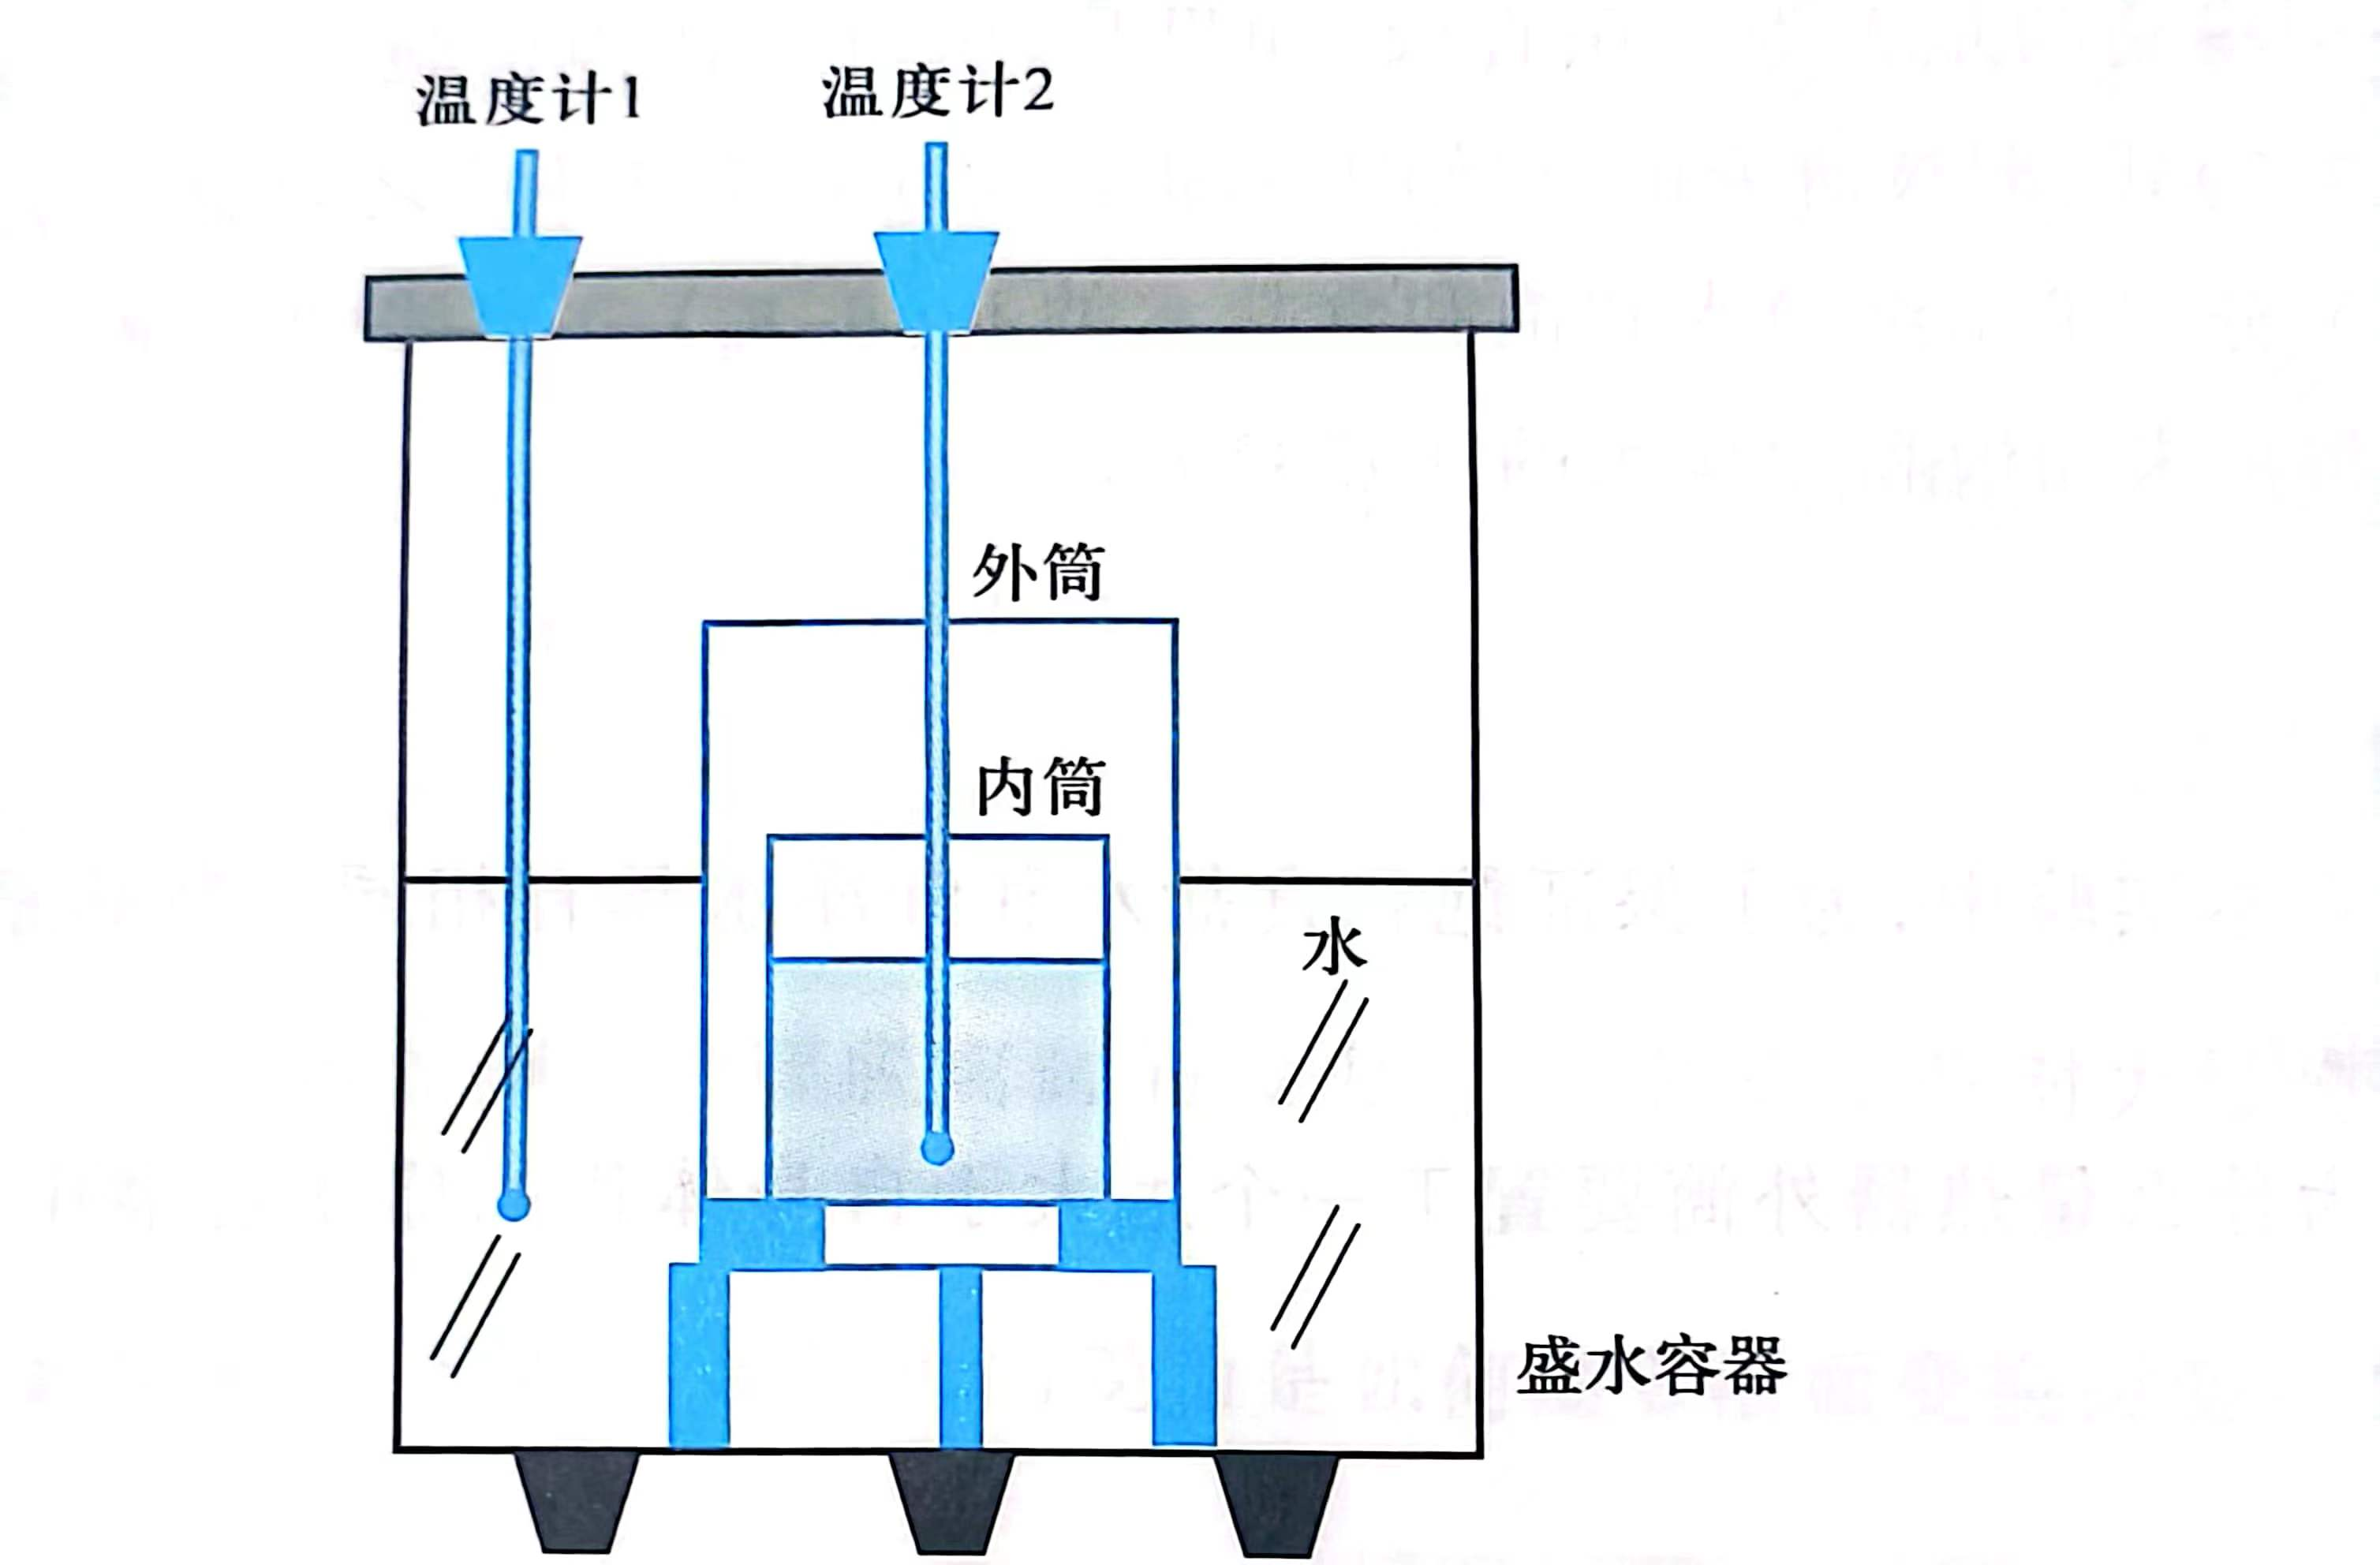
\includegraphics[width=0.5\textwidth,height=0.2\textheight]{qicai.jpg}
  \caption{专用量热器示意图}
\end{figure}

\section{实验内容及实验步骤}
  \subsection{仪器准备}
  (1)本实验所用量热器外筒远小于盛水盘,实验开始时将盛水盘盛上适当深度的水。

  (2)在恒温装置中配置饱和食盐水、纯净水并使两种液体的温度保持在7$^{\circ}C$左右。

  (3)用电子天平给量热器内筒称重。

  \subsection{测量饱和食盐水和纯净水的自然冷却过程}
  (1)量热器内筒盛上约占内简 2/3 体积的饱和食盐水,用电子天平称重后放入量热器外筒中,
  此时应保证饱和食盐水的温度比室温高10~15$^{\circ}C$。

  (2)每隔1min 记录一次饱和食盐水温度$\theta$和盛水容器冷却水的温度$\theta_{0}$,共测20 min。

  (3)将量热器内简从外筒中取出,用纯净水清洗。

  (4)量热器内简盛上约占内简2/3体积的纯净水,用电子天平称重后放入量热器外筒中.
  此时应保证饱和纯净水的温度比室温高10~15$^{\circ}C$,且纯净水与饱和食盐水的初温之差不超过1℃。

  (5)每隔1min记录一次纯净水温度$\theta$和盛水容器中冷却水的温度$\theta_{0}$,共测20 min。

  \subsection{数据处理}
  (1)在同一个直角坐标系中对纯净水及饱和食盐水分别
  作“$ln(\theta - \theta_{0}) - t$”图,
  检验分别得到的是否为一条直线。
  如果是,则可以认为检验了原理中推导的两个公式,即被研究的系统的冷却速率同系统与环境之间温度差成正比。

  (2)分别求出纯净水和饱和食盐水的$ln(\theta - \theta_{0}) - t$ 直线的斜率$S^{'} , S^{''}$,
  并通过比较法得出未知饱和食盐水的比热容$c_{x}$。
\newpage

\section{实验原始数据}
\begin{figure}[H]
  \centering
  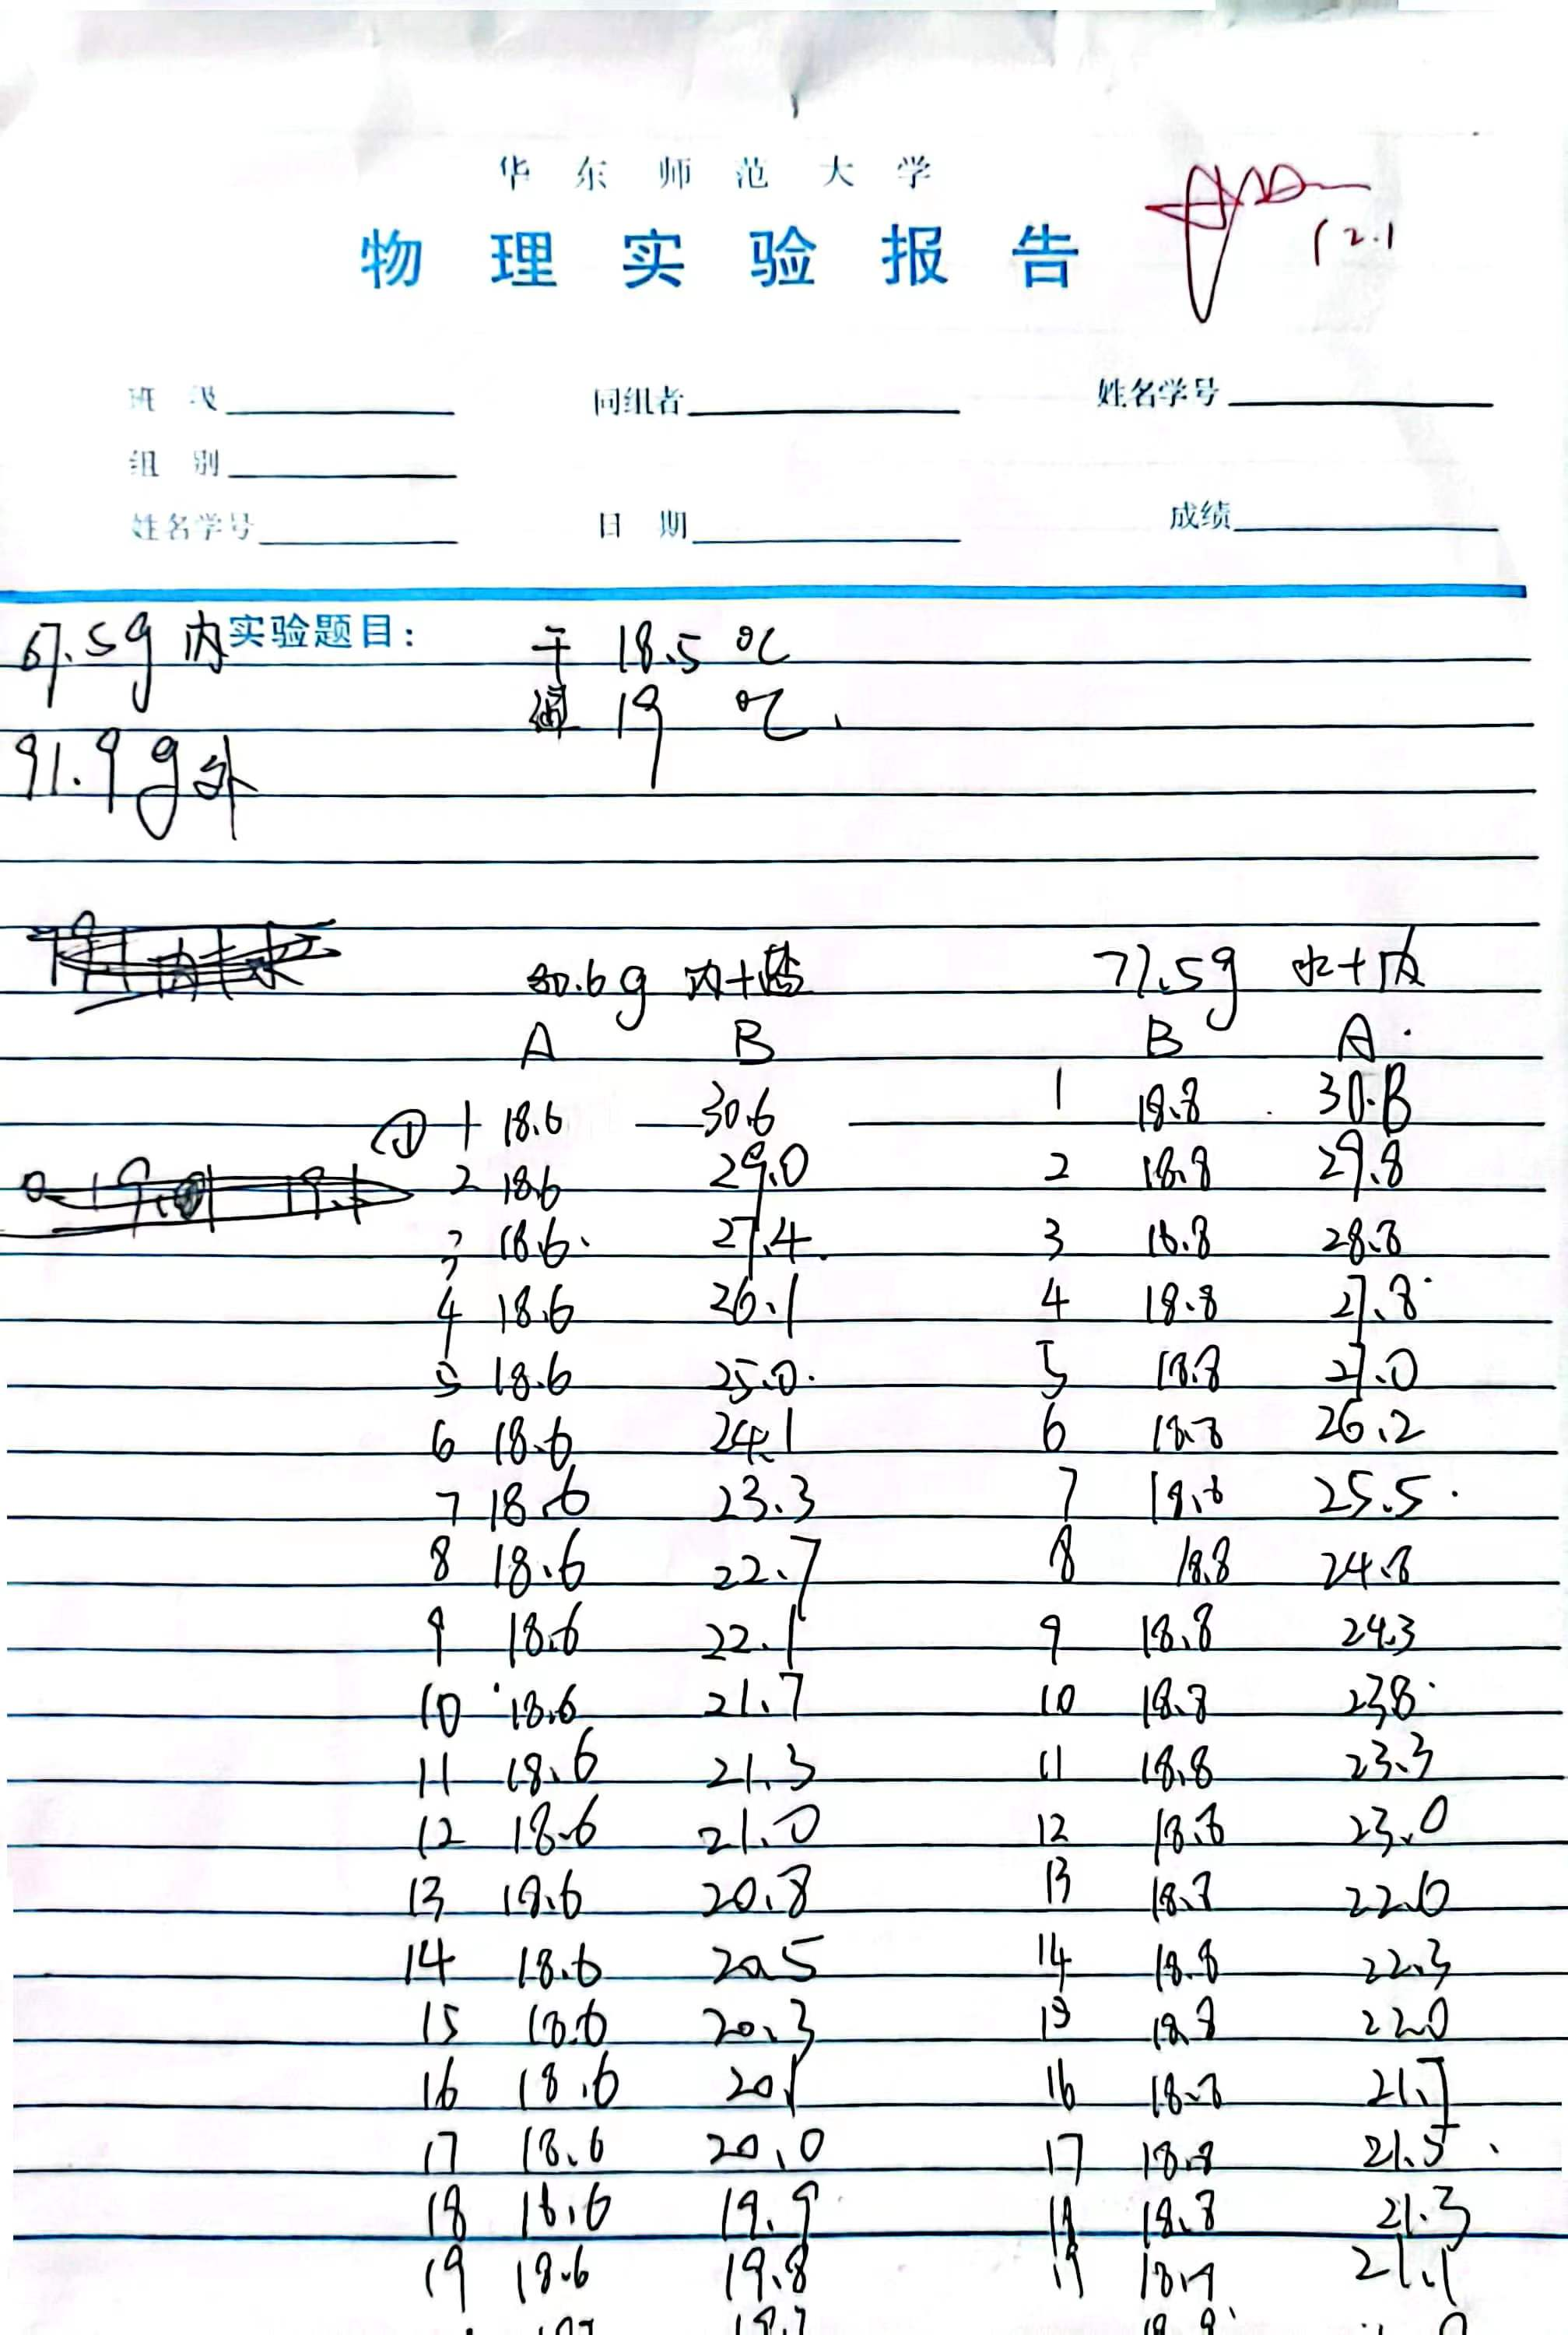
\includegraphics[width=0.9\textwidth,height=0.8\textheight]{yuanshishujv.jpg}
  \caption{实验原始数据}
\end{figure}
\newpage


\section{实验数据处理}
实验数据处理后的图像如下图所示:
\begin{figure}[H]
  \centering
  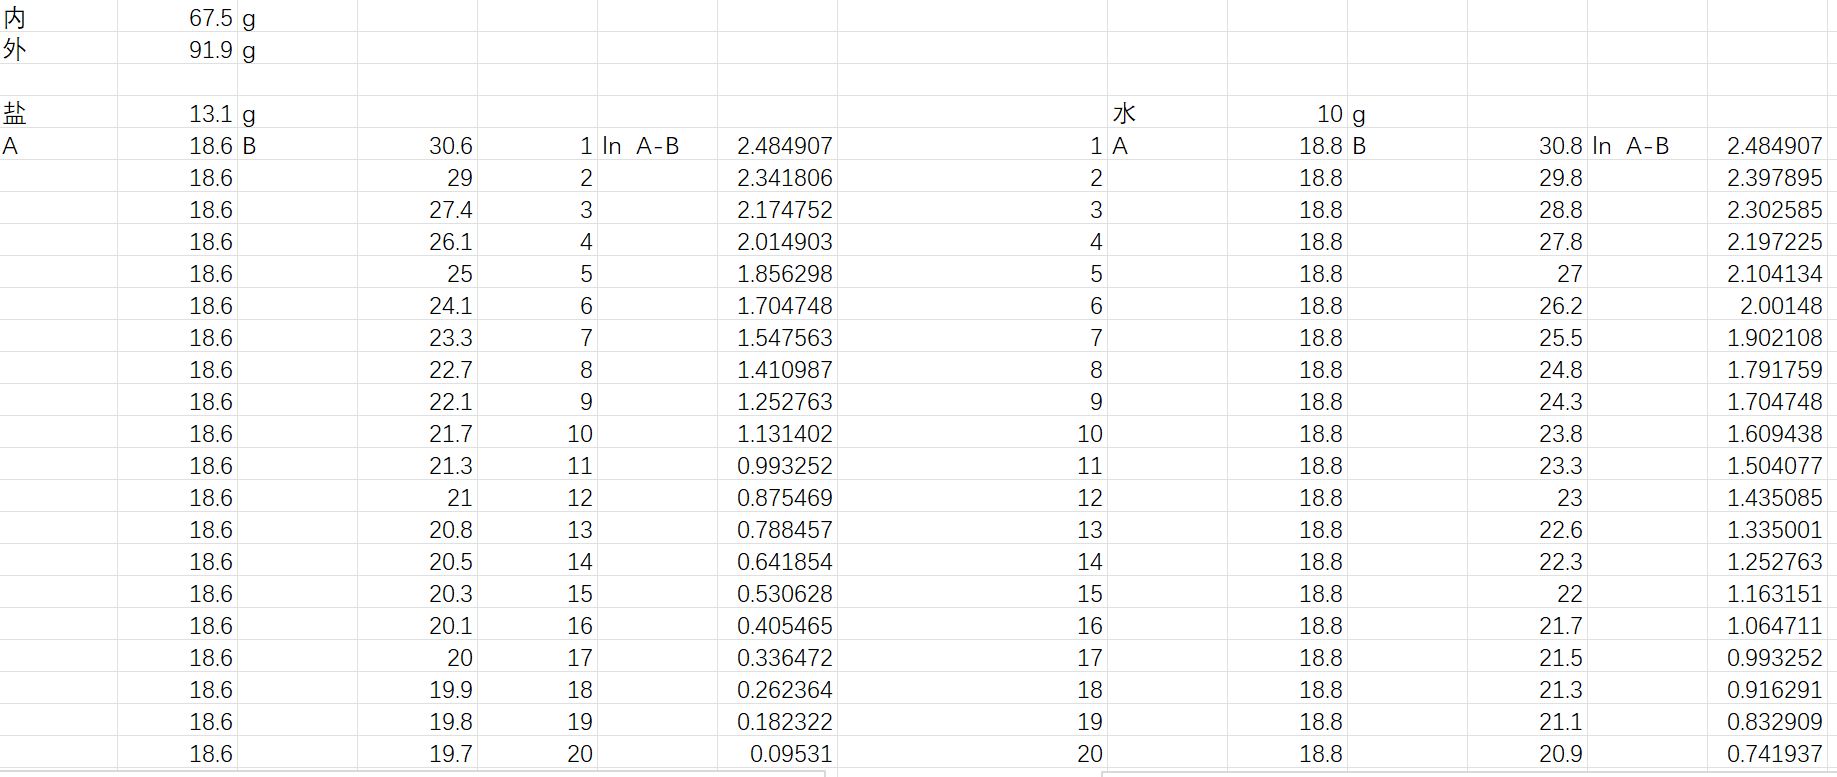
\includegraphics[width=0.9\textwidth,height=0.5\textheight]{shujvchuli.png}
  \caption{实验数据处理}
\end{figure}

此图为实验数据的初步处理,计算了$ln(\theta - \theta_{0})$ 的值的大小和后续所需要的数据。

\begin{figure}[H]
  \centering
  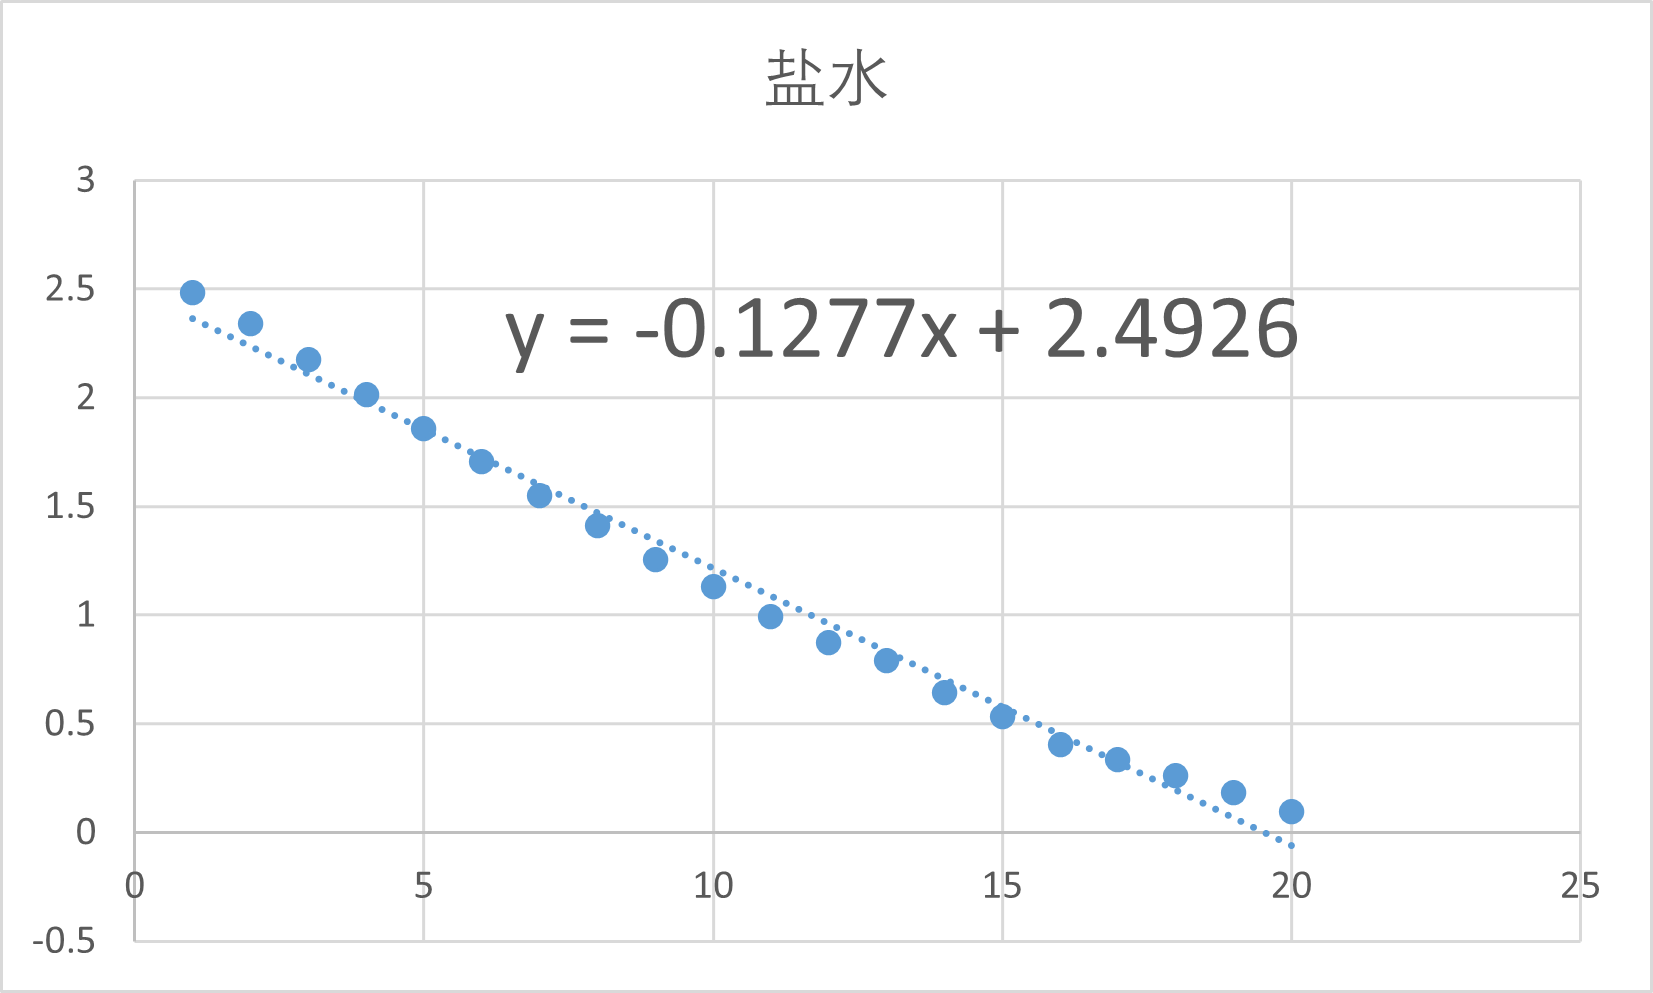
\includegraphics[width=0.5\textwidth,height=0.2\textheight]{nacl.png}
  \caption{盐水图像}
\end{figure}

此图为盐水的数据图像化后的结果,可以从图中得到拟合直线的斜率等信息。

\begin{figure}[H]
  \centering
  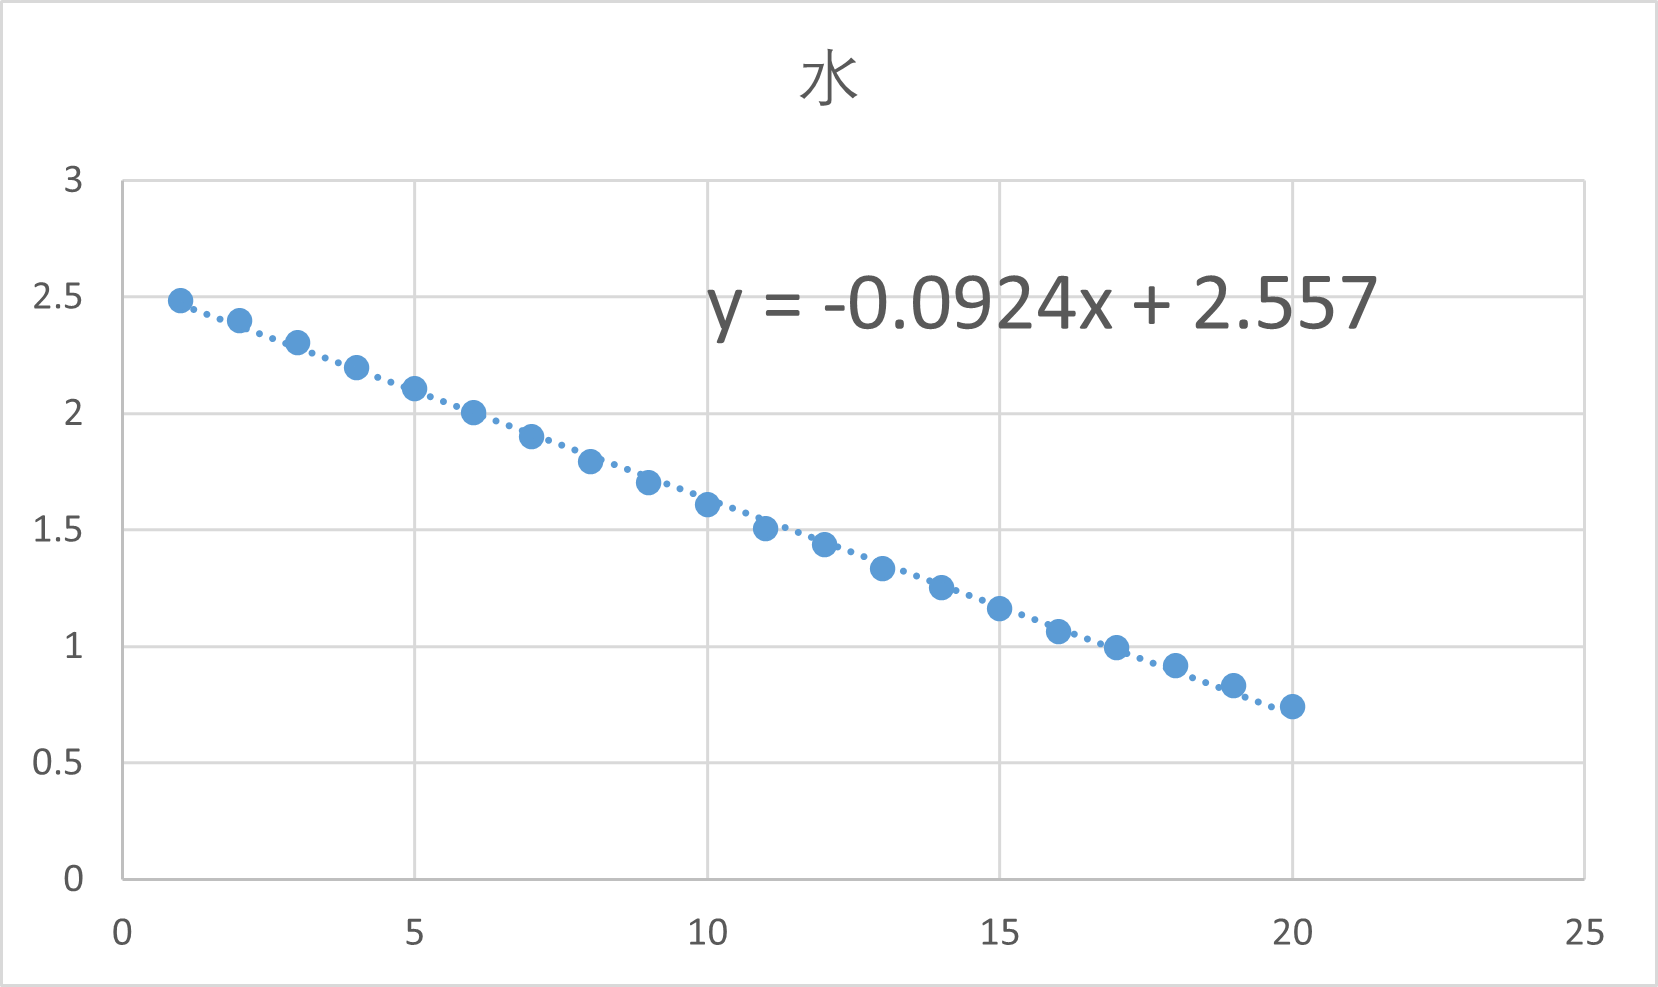
\includegraphics[width=0.5\textwidth,height=0.2\textheight]{h2o.png}
  \caption{纯水图像}
\end{figure}

此图为纯水的数据图像化后的结果,可以从图中得到拟合直线的斜率等信息。

最终通过计算得到实验测得的饱和盐水溶液的比热容为1.554$J / (g \cdot K)$。

实验得到的食盐水的比热容比较小,可能由于浓度比较高导致的。实验中的误差主要来自于实验器材本身和
周围环境的变化。


\section{思考题}
  \subsection{思考题一}
  实验中确保饱和食盐水和纯净水都放置在相同类型、相同材质和相同容积的容器中,
  以减少容器对实验结果的影响。同时还使饱和食盐水和纯净水的起始温度相同。
  并提供尽量相同的实验环境条件。
  并且为了防止液体在实验过程中因为蒸发或溢出而减少,这可以通过适当盖子覆盖容器来实现。

  \subsection{思考题二}
  这样有利于稳定温度,减少外部温度变化对实验结果的影响。
  同时保证散热平衡。稳定外部散热系数。

\section{实验中个人的思考与感想}
  \subsection{对于实验个人观点}
  实验过程非常简单,只需要选择合适的测量温度然后等待温度自己慢慢下降就可以,基本没什么难度。
  而实验的原理也比较容易理解,主要通过的就是已知水的比热容这一点,通过饱和食盐水和纯净水降温
  速度的比较最终得到相对于水的比热容,也就可以得到饱和食盐水的比热容。

  \subsection{实验中的总结}
  通过测量饱和食盐水和纯净水在从一定温度在20min内的降温,利用比较法,得到饱和食盐水的比热容
  约等于1.554$J / (g \cdot K)$。
\end{document}
